% !TeX spellcheck = en_GB
\chapter{Results}
\section{LWC and LWP from MEPS}%\hfill} 
\label{app:LWP_MEPS}

%%% image LWC Retrieval MEPS comparison %%%%%%%%%%%%%%%%%%%%%%%%%%%%%%%%%%%%%
\begin{figure}[t]%\ContinuedFloat
	\centering
	% 21/12
	\begin{subfigure}[t]{0.85\textwidth}
		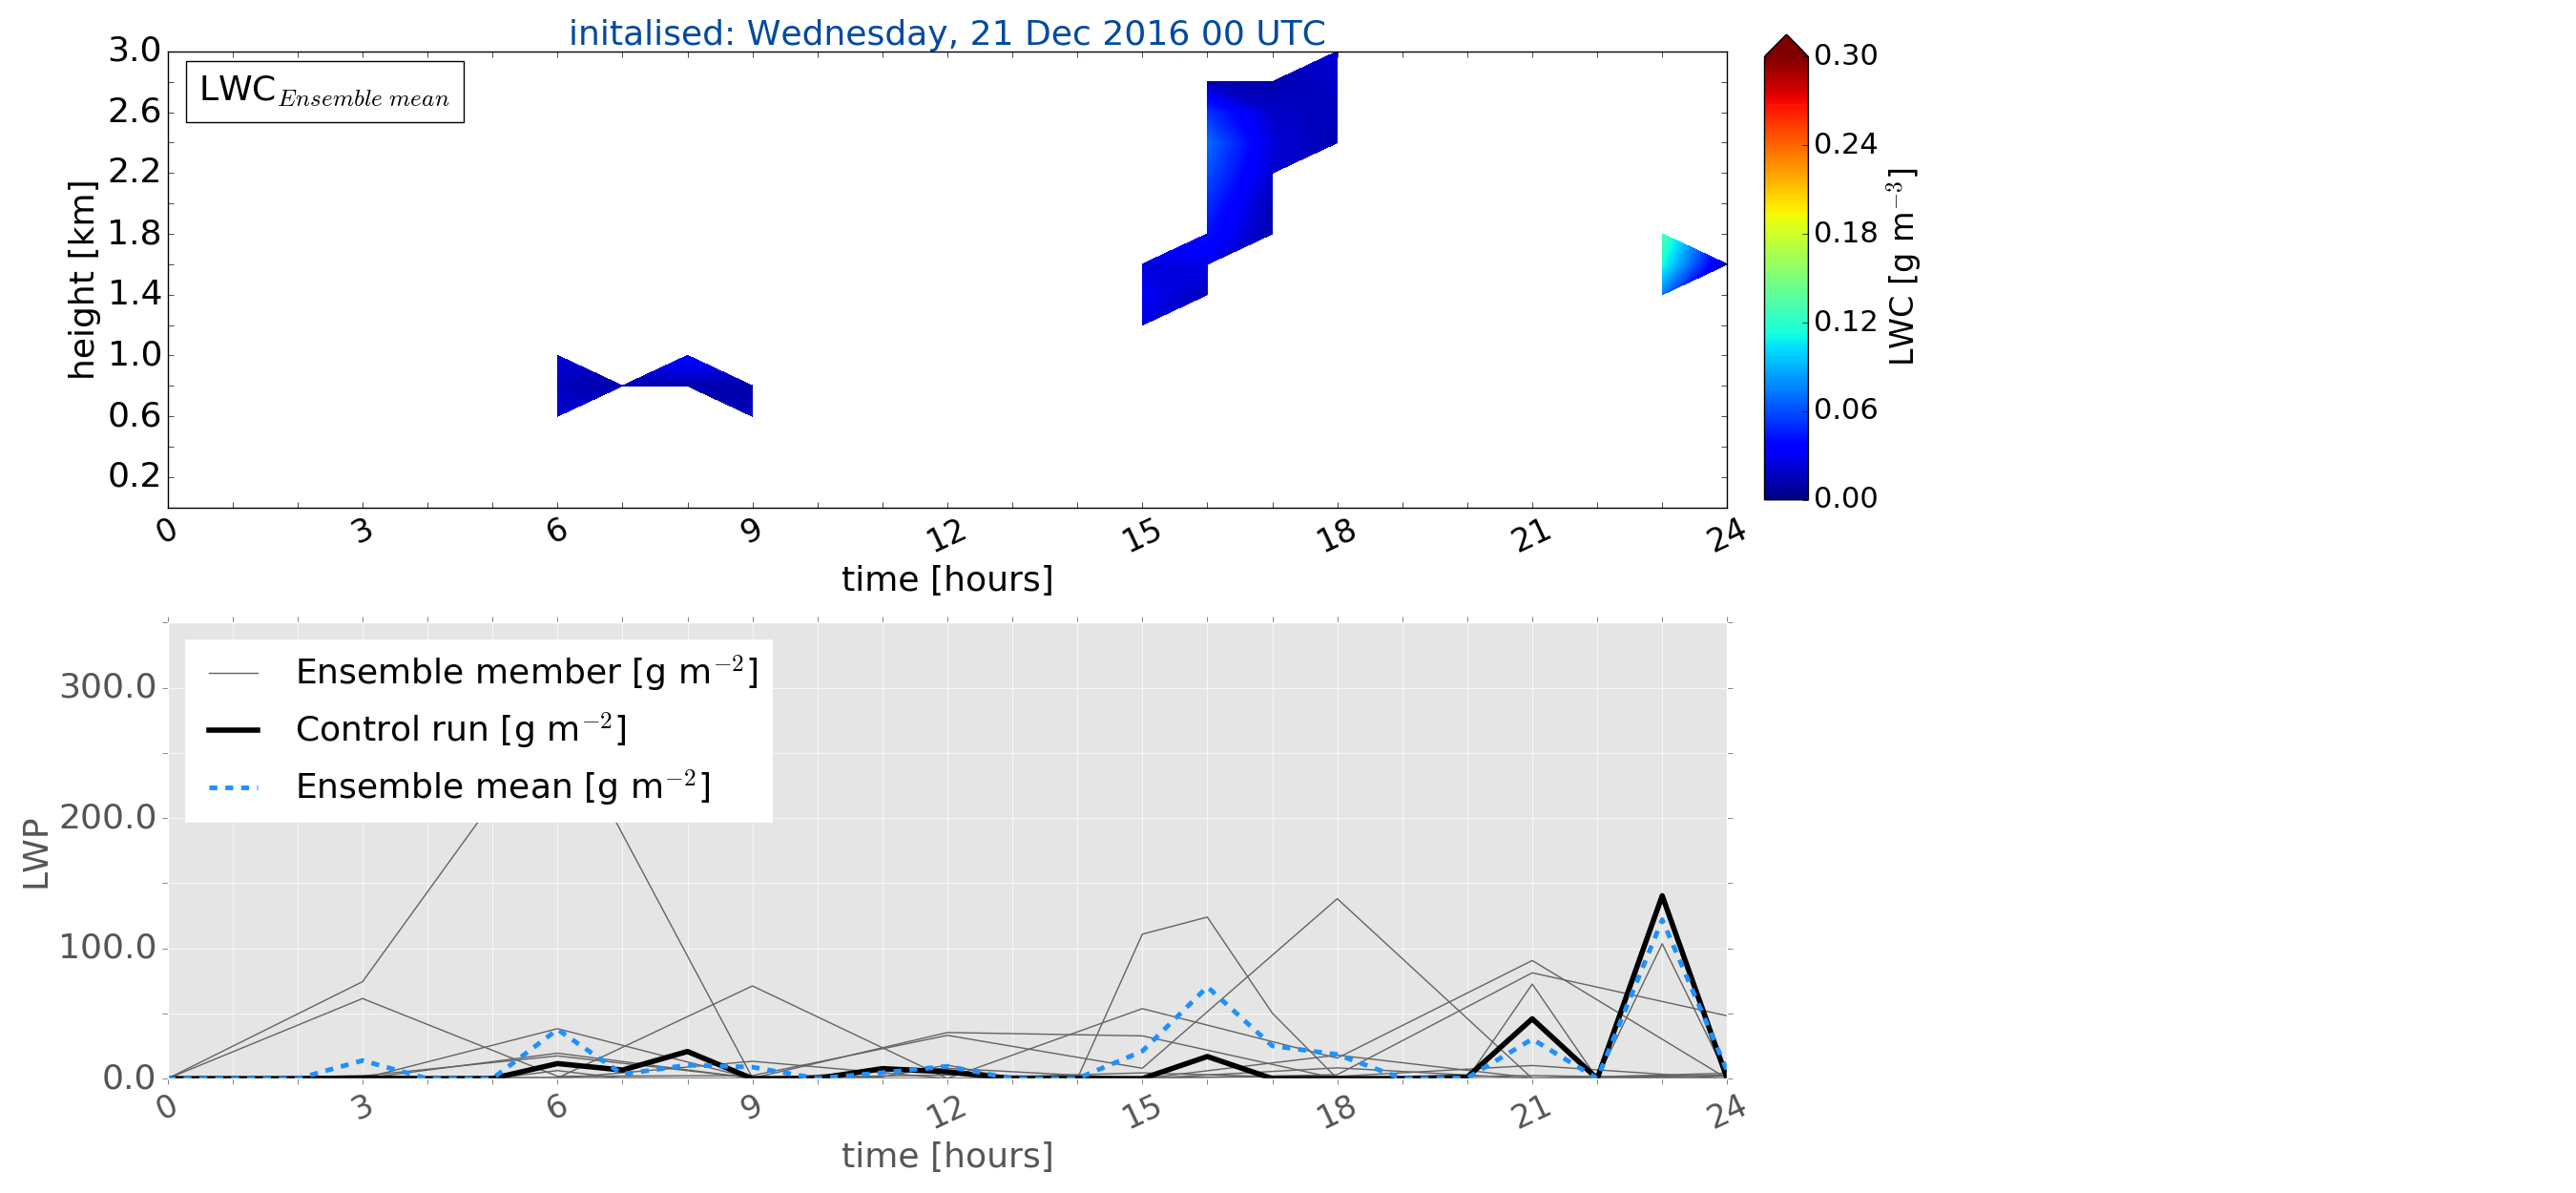
\includegraphics[trim={.5cm 0.5cm 27cm .5cm},clip,width=\textwidth]{./fig_LWC/20161221}
		\caption{}\label{fig:LWC21}
	\end{subfigure}
	\centering
	% 22/12
	\begin{subfigure}[t]{0.85\textwidth}
		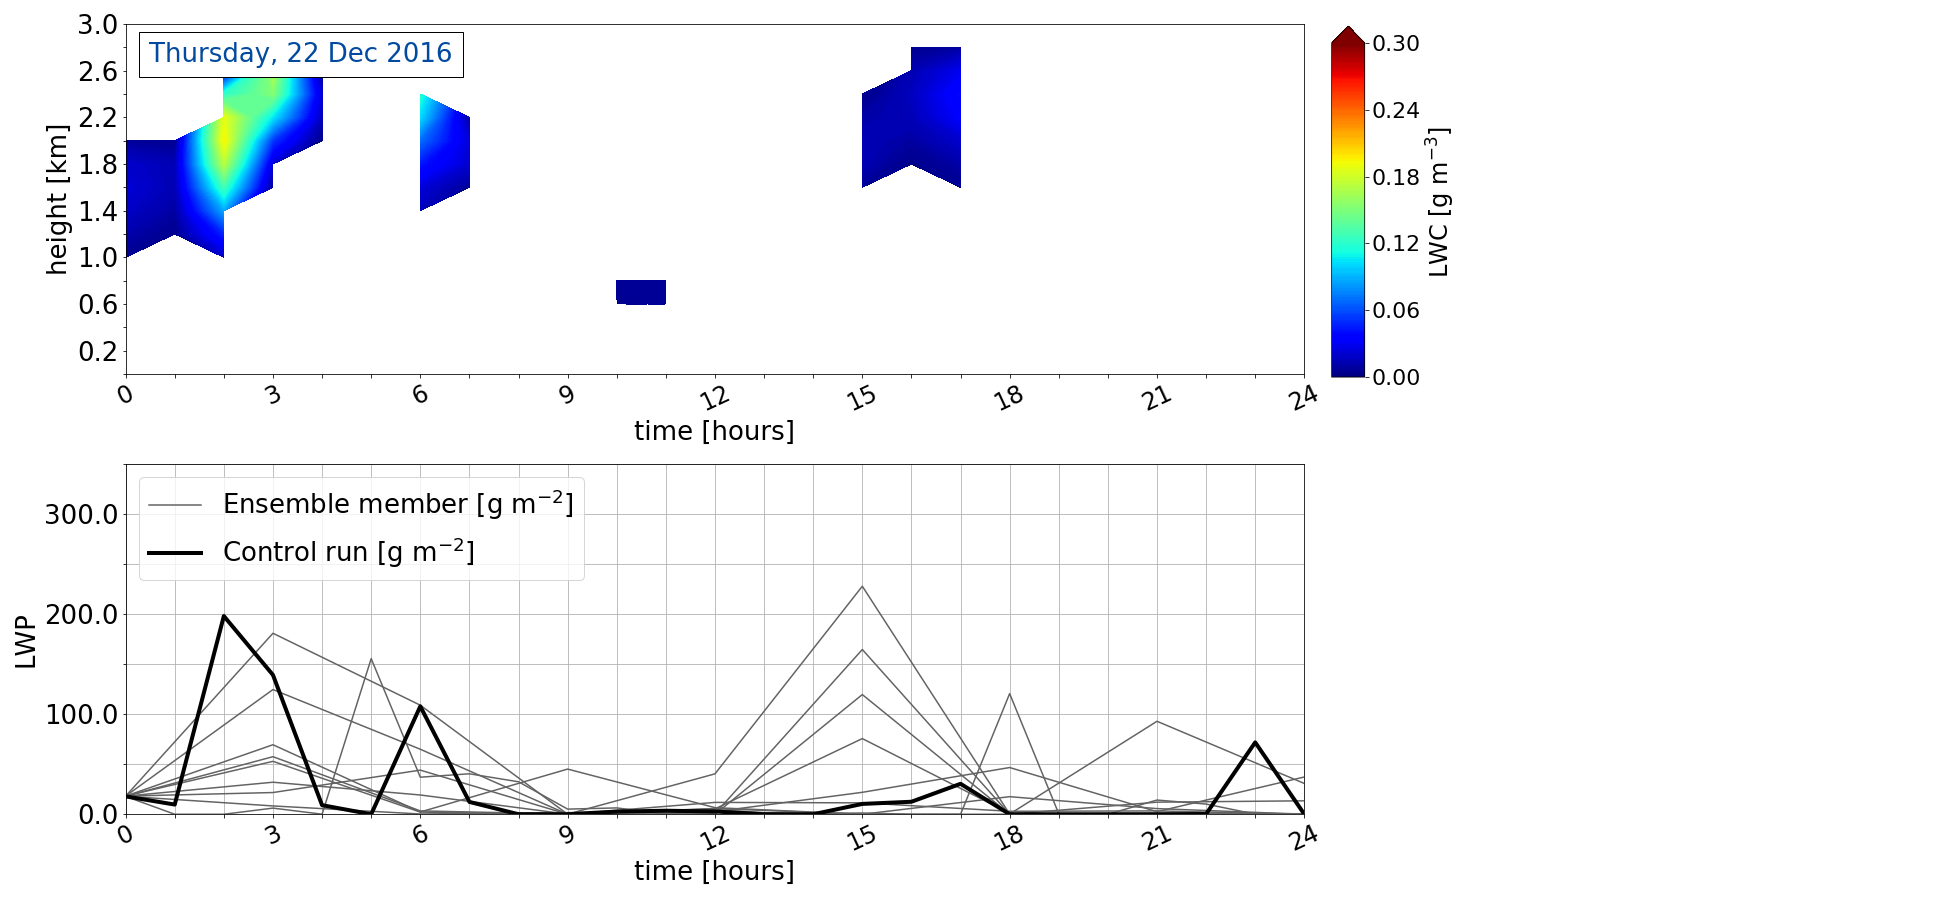
\includegraphics[trim={0.5cm 0.5cm 27cm .5cm},clip,width=\textwidth]{./fig_LWC/20161222}
		\caption{}\label{fig:LWC22}
	\end{subfigure}
	%\end{figure}
	%\begin{figure}\ContinuedFloat
	\centering
	% 23/12
	\begin{subfigure}[t]{0.85\textwidth}
		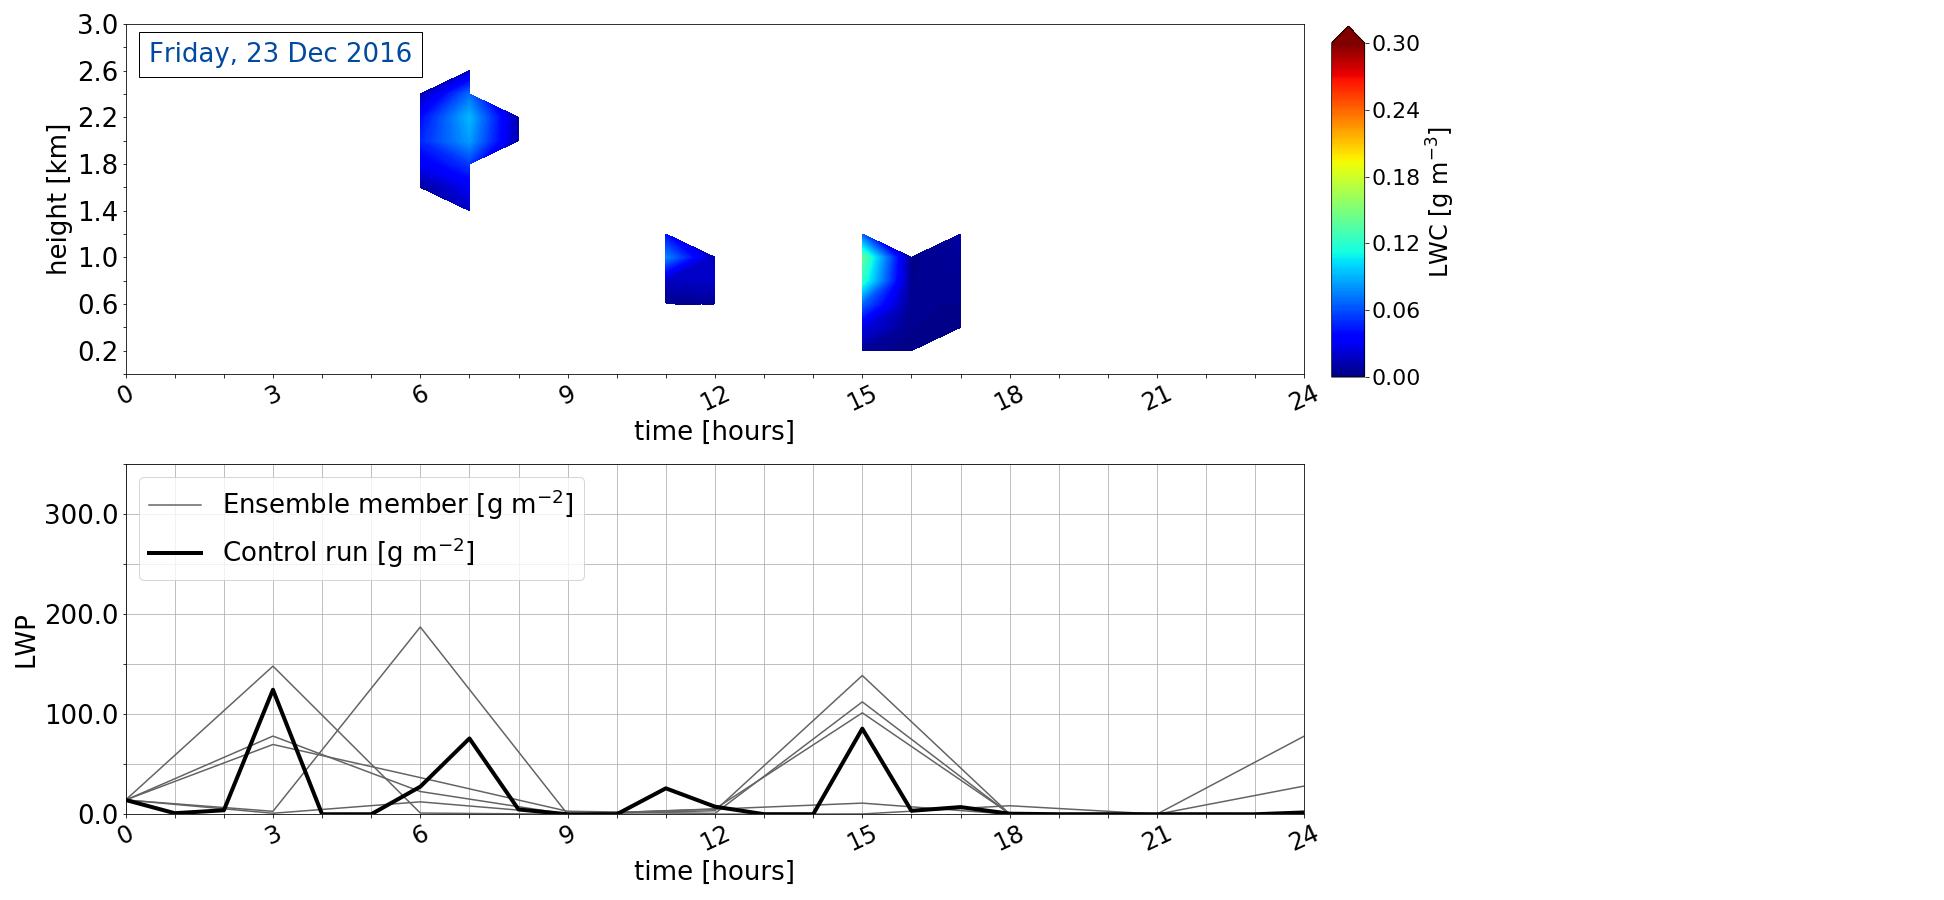
\includegraphics[trim={0.5cm 0.5cm 27cm .5cm},clip,width=\textwidth]{./fig_LWC/20161223}
		\caption{}\label{fig:LWC23}
	\end{subfigure}
\end{figure}
\begin{figure}\ContinuedFloat        
	\centering
	% 24/12
	\begin{subfigure}[t]{0.85\textwidth}
		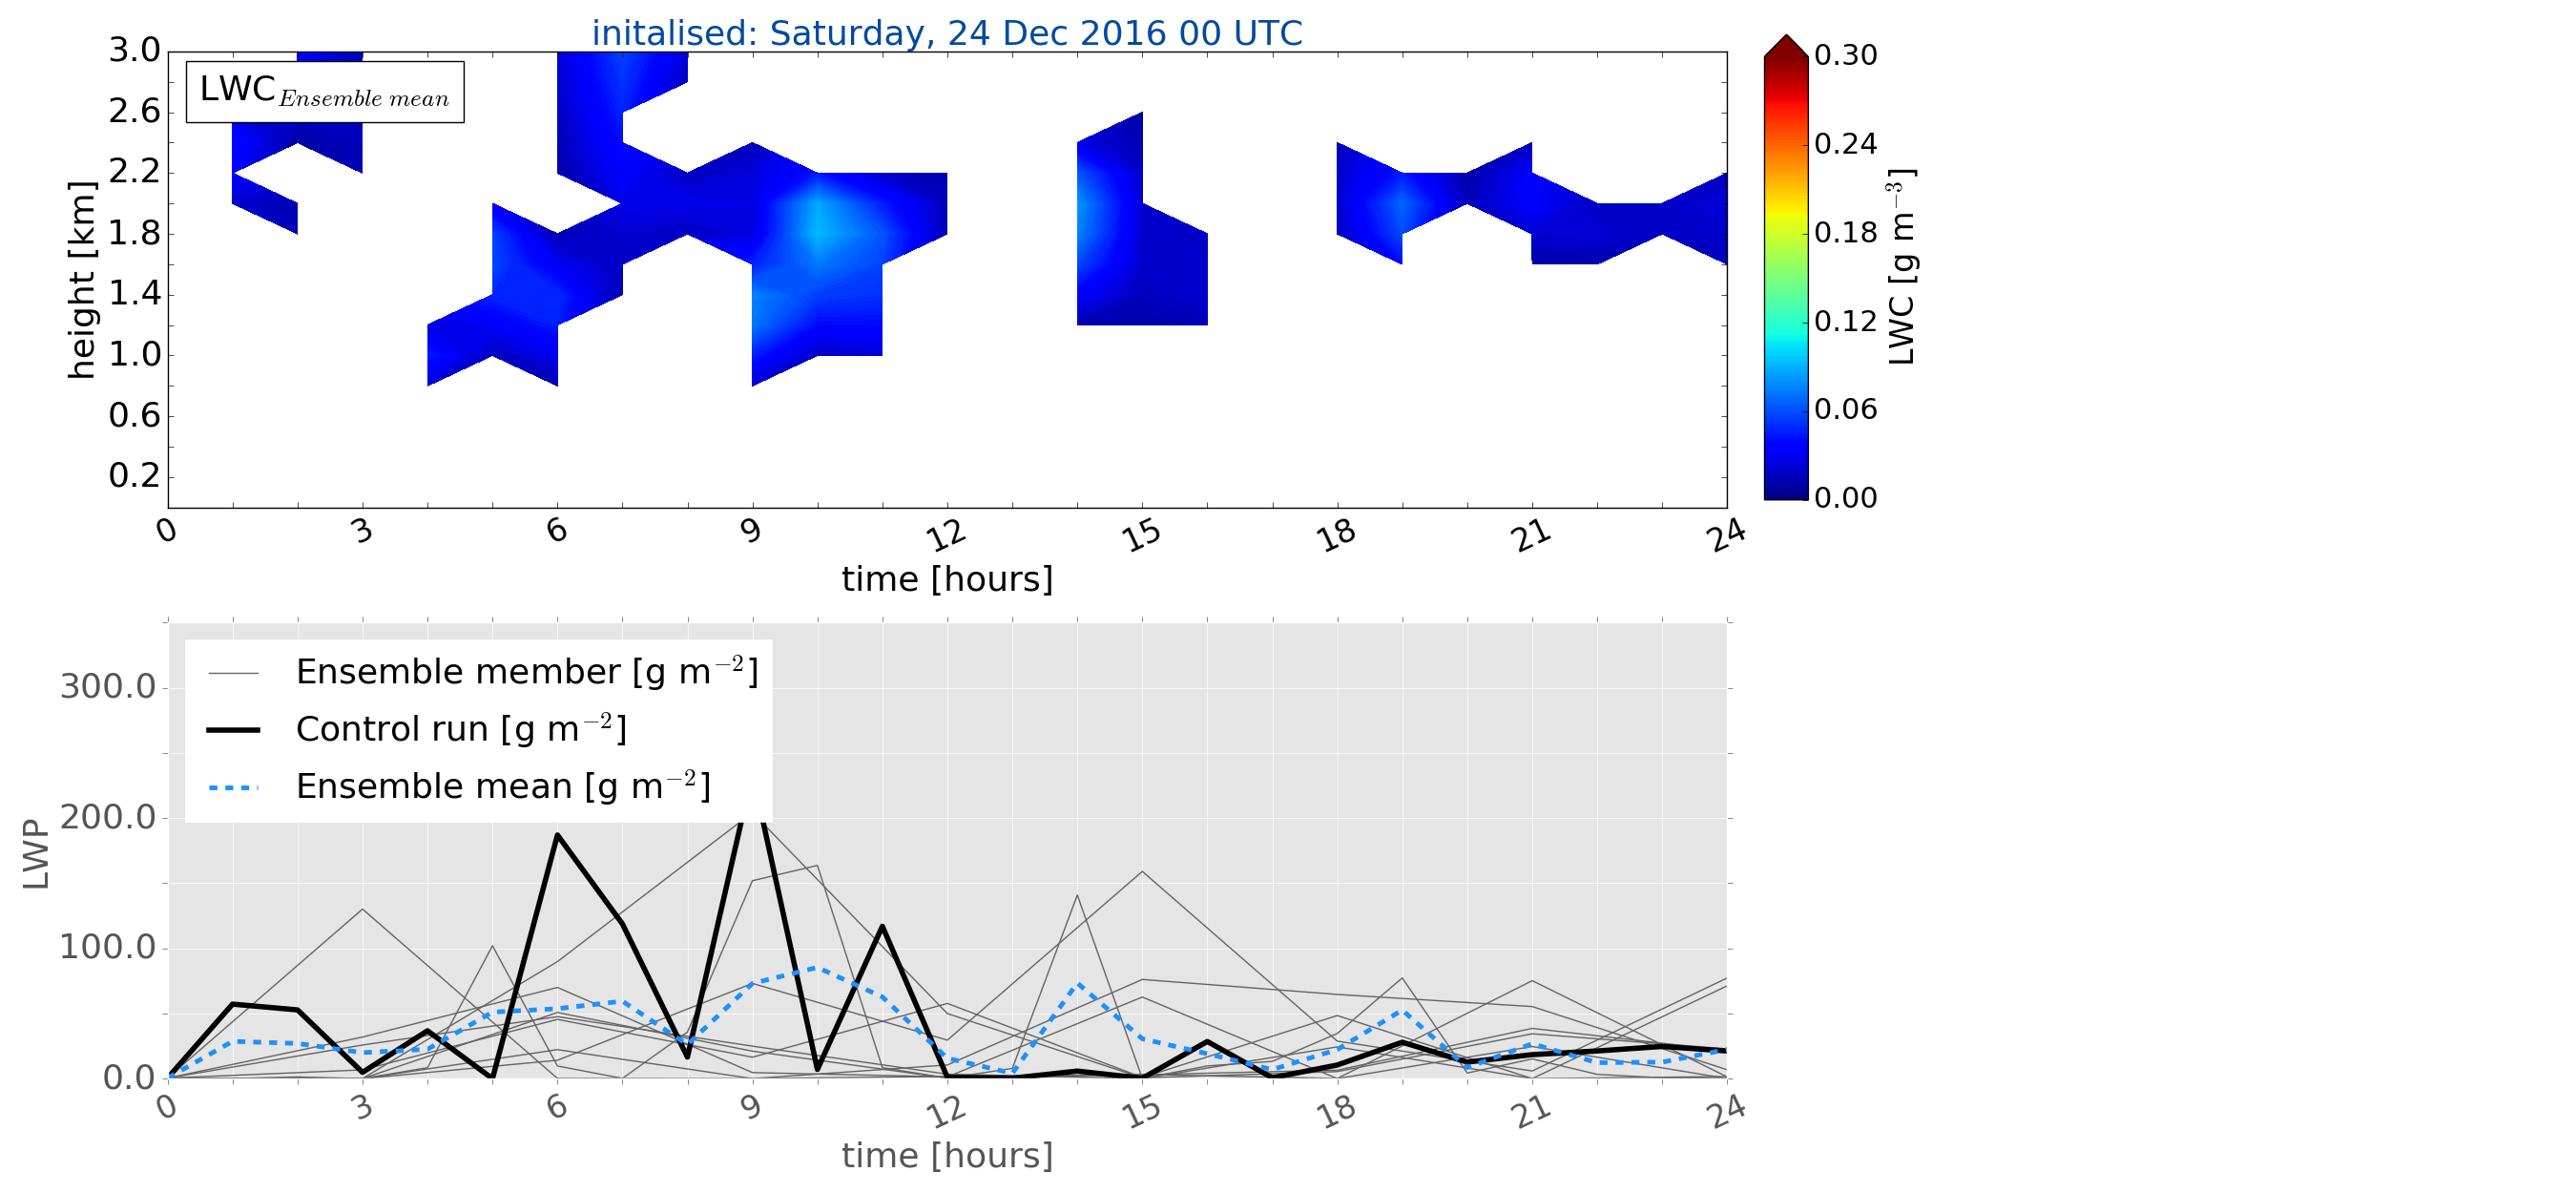
\includegraphics[trim={0.5cm 0.5cm 27cm .5cm},clip,width=\textwidth]{./fig_LWC/20161224}
		\caption{}\label{fig:LWC24}
	\end{subfigure}
	
	\centering
	% 25/12
	\begin{subfigure}[t]{0.85\textwidth}
		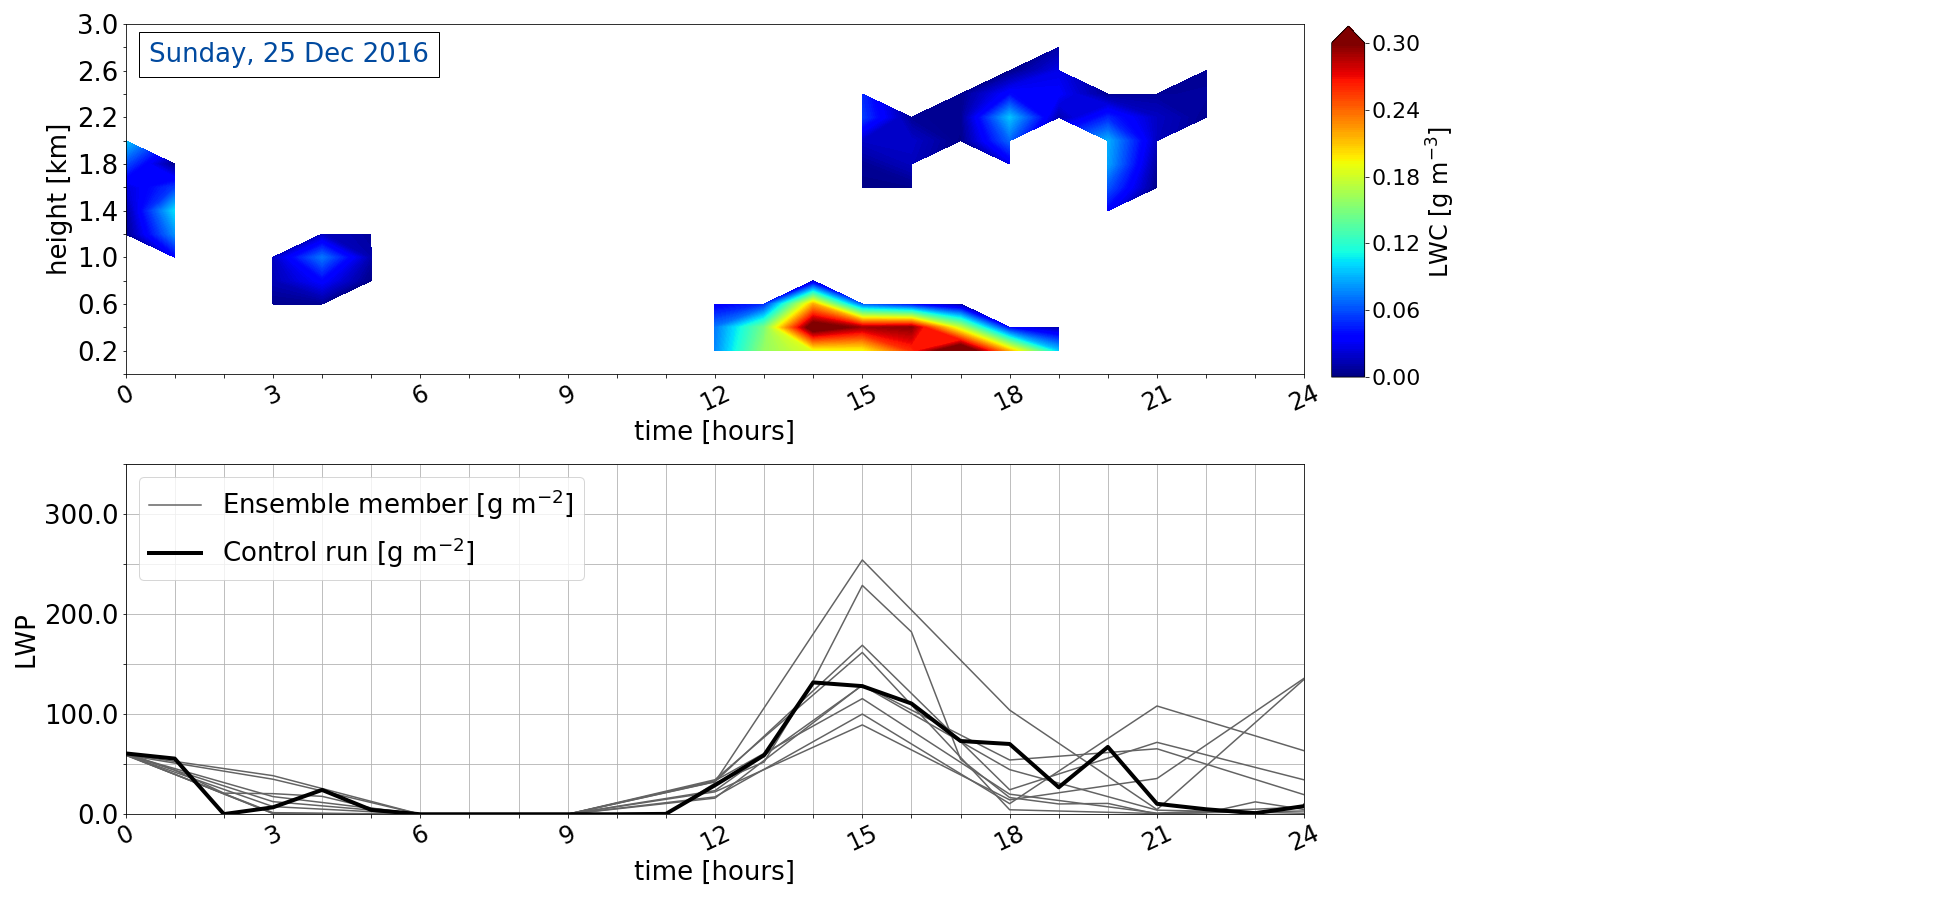
\includegraphics[trim={0.5cm 0.5cm 27cm .5cm},clip,width=\textwidth]{./fig_LWC/20161225}
		\caption{}\label{fig:LWC25}
	\end{subfigure}
	%\end{figure}
	%\begin{figure}\ContinuedFloat
	\centering
	% 26/12
	\begin{subfigure}[t]{0.85\textwidth}
		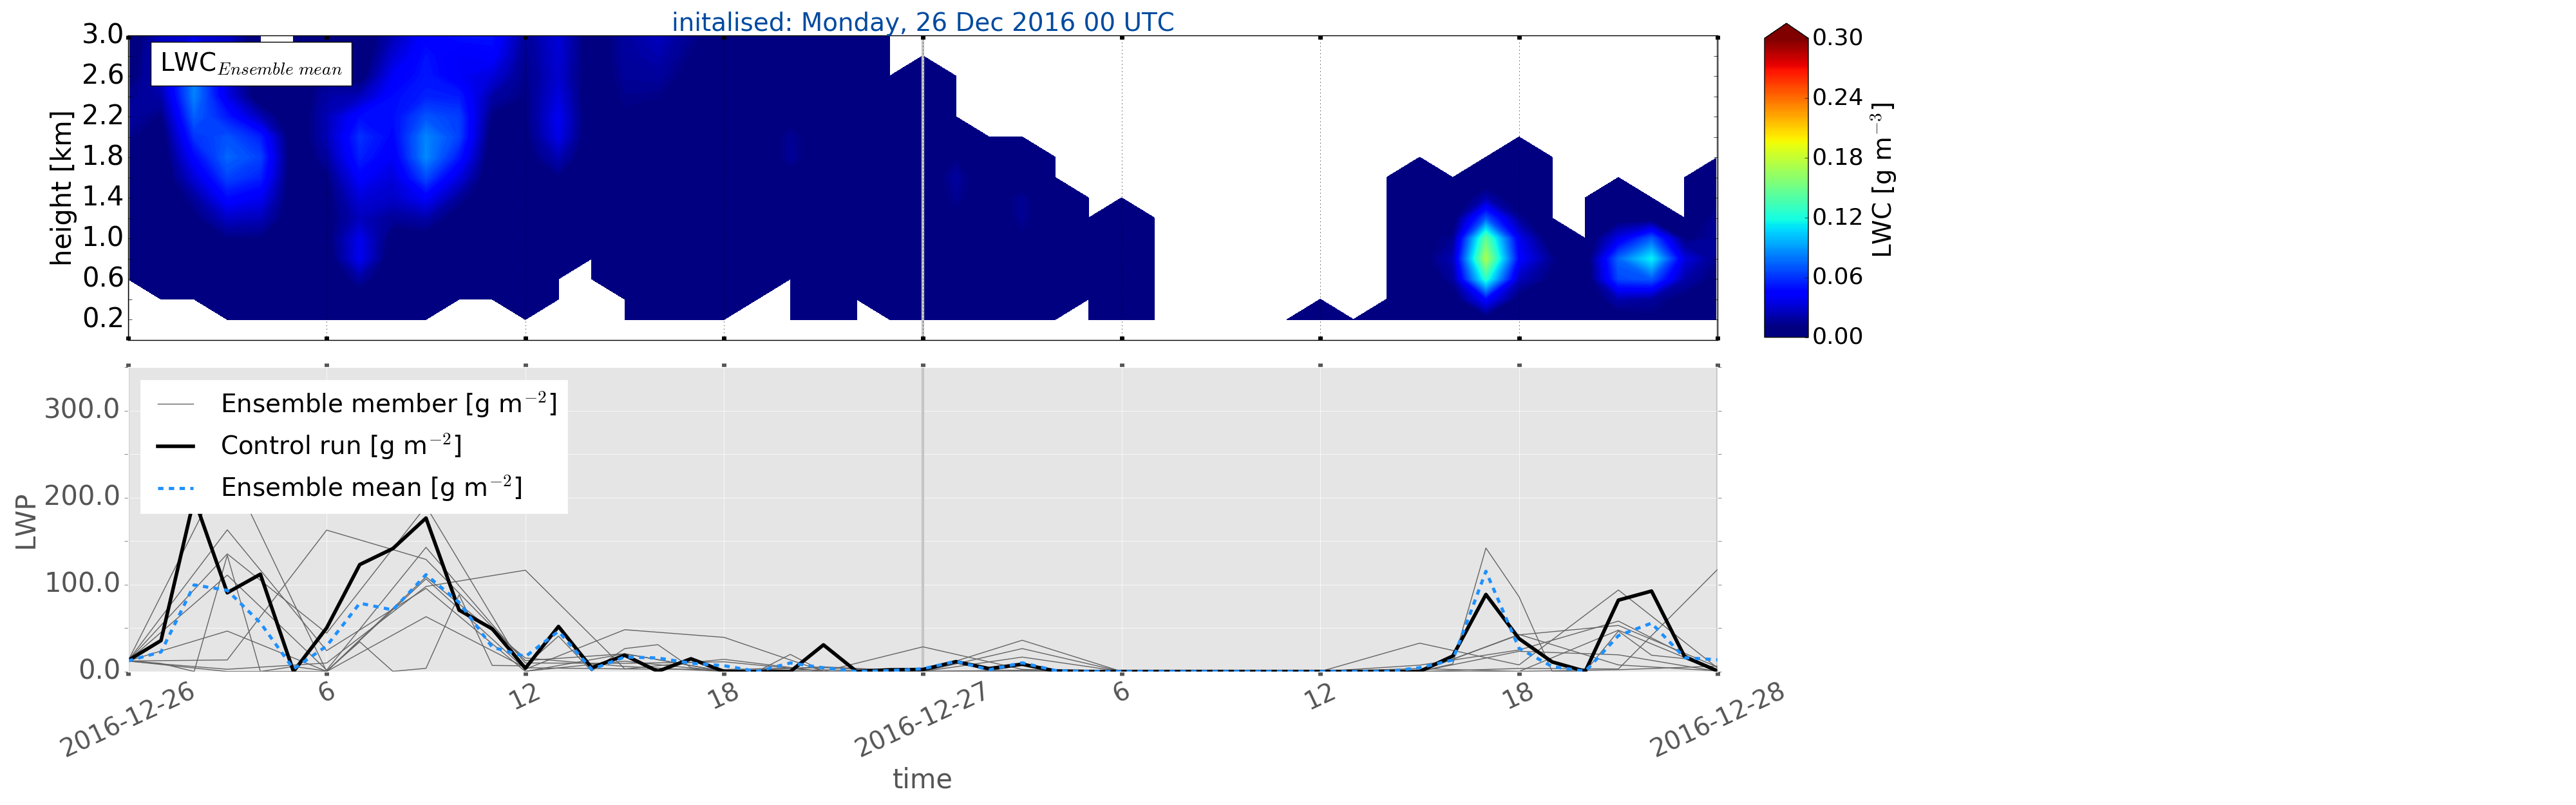
\includegraphics[trim={0.5cm 0.5cm 27cm .5cm},clip,width=\textwidth]{./fig_LWC/20161226}
		\caption{}\label{fig:LWC26}
	\end{subfigure}
	\caption{Upper panel: \SI{200}{\metre}-averaged LWC ensemble mean forecast from MEPS. 
		Lower panel: LWP from MEPS, initialised at \SI{00}{\UTC}. Black line represents the deterministic forecast, the doted blue line the ensemble mean and the grey lines the nine perturbed members.}\label{fig:LWC}
\end{figure}
%%%%%%%%%%%%%%%%%%%%%%%%%%%%%%%%%%%%%%%%%%%%%%%%%%%%%%%%%%%%%%%%%%%%%%%%%%
